\chapter{Methods\label{cha:methods}}

In this chapter we describe our implementation of the game Breakthrough and the methods for training a neural network to play the game Breakthrough, described in Chapter \ref{cha:background}. The training process uses MCTS described in Section \ref{sec:mcts} to guide its training. We outline the architecture used in the neural network.

The training algorithm is a reinforcement learning self-play algorithm based on previous work by DeepMind (CITE ME).

\section{Implementation}

In this section we will take a brief look at the implementation of the game Breakthrough, how we model its state representation, and the pseudocode for training.

\subsection{Breakthrough}

In order for a neural network to be able to use input, that input needs to be numeric. We model the board in gamethrough with a single $NxM$ array with three values $\{-1,0,1\}$. Where each $x,y$ index on the board represents what value is on the board at the time, $-1$ represnts a white piece, $0$ represents an empty square, and $1$ represents a black piece.

A action vector is coupled with each state, the action vector is a $3$-dimensional matrix where the lengths of the dimensions are $row x columns x 6$ and each index of the vector $X,Y,Z$ represents an action moving from cell $x,y$ moving to the direction $z$. The directions are as follows $0$ represents moving upwards and to the left diagonally on the board, $1$ upwards, and $2$ upwards and to the right diagonally, $4$ downwards and to the left diagonally, $5$ downwards, and lastly $6$ downwards and to the right diagonally.

\subsection{Selfplay}



\section{Neural Network Architecture}

The neural network architecture we opted to use was a single convolutional layer with a ReLU activation function, followed by 5 residual layers each containing two layers of convolution, batch normalization and a ReLu activation. Lastly a split policy/value head, where the output of the last residual layer is split into two different outputs. The policy head are two layers: first a final convolutional layer, and last a fully connected layer with a \textit{log softmax} layer. The value head, consists of three layers: first a convolutional layer, then a fully connected layer, and lastly a fully connected layer with a \textit{tanh} activation function. The Figure \ref{fig:nnarch}. depicts the architecture.

\begin{figure}[]
    \centering

    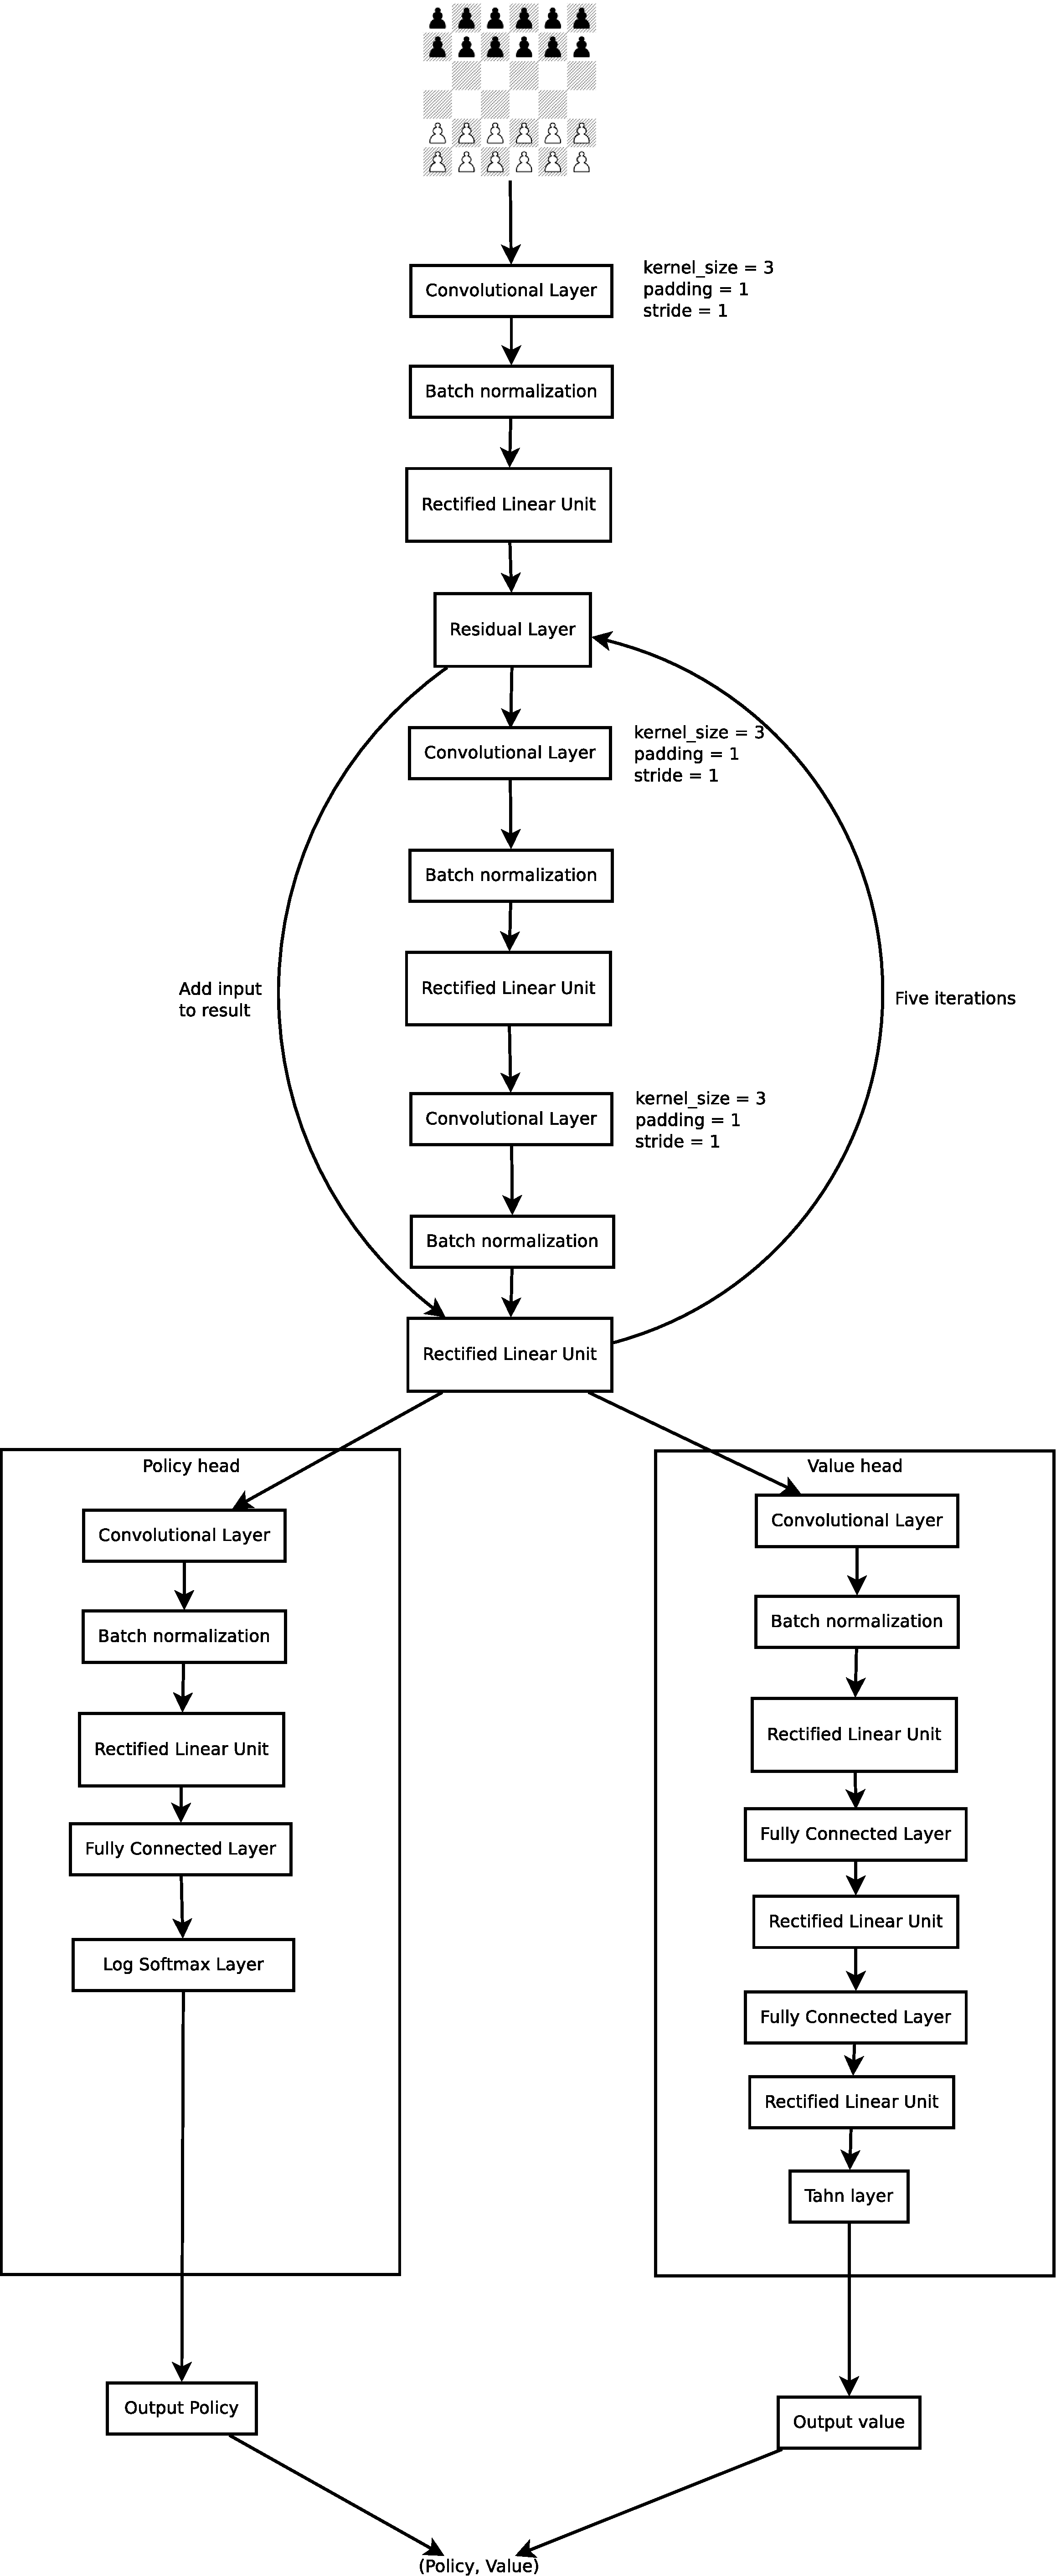
\includegraphics[width=0.65\textwidth]{graphics/test}
    
    \caption{Neural Network Architecture}
    \label{fig:nnarch}
\end{figure}

\subsection{Convolutional Layers}

It is important to understand why we use convolutional layers when dealing with board games as convolution is often associated with image. This is because a convolutional layer is focused on merging multiple input parameters to a single neuron, making it an input parameter for the next layer representing the locality around the center point of the original input. Playing the game of Breakthrough, a piece in only able to capture pieces in its immediate vicinity. This lead to the selection of a convolutional kernel with the size of $3x3$ and a stride of $1$.

The knowledge of each piece moves isn't enough to represent the whole gamestate within the neural network. This is why we use multiple residual layers with convolution. These residual layers stack convolutions on each other making the final convolution represent the locality of all the other localities, allowing the neural network to have a representation of the whole gamestate in its parameters.

The selection of parameters was done for these reasons as well as to most closely resemble the architecture described in AlphaZero.

\subsection{Residual Layers}

The residual layers as a concept remember the output of the previous layer and add the results of the residual layer and the previous layer together. On a higher level this leads to the internal representation of the neural network to maintain the whole game boards in its representation, s.t. two areas that are far away from each other maintain the same level of locality as two that are close.

Why we use a residual layer for applying a convolution layer multiple times is to gain locality of the whole game board. A residual layer applies a function like this $res(x) = x + l(x)$ where $l(x)$ is the function of the layer, commonly a convolutional layer.

\subsection{Policy Head}

The policy head of the neural network returns a vector of the size of the action space $w * h * 6$ where $w$ is the width of the board $h$ is the height of the board and $6$ represents the six cardinal direction pawns can move (straight, and diagonally both left and right for the first player, and backwards for the second player). The vector is then masked s.t. the values representing moves that can not be played on the board are given the value of $0$.

\subsection{Value Head}

The value head of the neural network returns a single value representing the predicted value of the neural network. This predicted value is trained to be the end value of the game after taking the predicted move.

\subsection{Self-play}

To train the neural network to play Breakthrough we initialize two neural networks $N_1$ and $N_2$ 
with random weights. Then we let $N_1$ play against itself using MCTS to direct its training. 
While playing against itself the neural network gathers data for it to train with. 

The data collected is $(\pi, \tau, p, v)$, where $\pi$ is the action probabilities provided by 
MCTS for $N$ iterations, $\tau$ is the reward for the whole episode, $1$ if white wins,
$-1$ if black wins, $p$ is the policy vector
from the neural network, and $v$ is the predicted reward of the game by the neural network.

This data collection trains the neural network in such a way that it is a function approximation for a single state to return the values that would have been returned from applying MCTS for $N$ iterations.


\subsection{Loss Function}

The data collected is backpropagated through the NN moving the weights to the direction of this 
loss function $l = (p * \pi) + (\tau - v)^2$ for each state the NN encountered during self-play.

\section{Explainable state representations}

In this section we describe the 

\subsection{Testing With Concept Activation Vectors}

Once the neural network has learned to play the game of Breakthrough, we examine its internal state w.r.t HLC's that we understand. The first examined HLC is numbers advantage, that is, the number of pieces that a player has over his opponent. The higher level idea to a human player would be that they are in a better position since they have more pieces.

To examine the higher level component we take a look at the internal state of the neural network itself. To do this we take a state, we run the state through the neural network, and while the state is propagating through the network we select a layer to split the network, we call that layer $l_{split}$. At that point in time the state is a mutated vector $l_{split}(l_{split-1}(...l_0(state)))$ of the initial state. We save that vector as a point in the N-dimensional space that it represents, and once we've gathered enough points in that N-dimensional space we're able to train a linear classifier using the HLC as a label. We train a Stochastic Gradient Descent classifier, from the SKLearn library, to construct a hyperplane that splits the space into two binary states, one that contains the HLC and another that doesn't. 
\begin{figure}[]
    \centering
    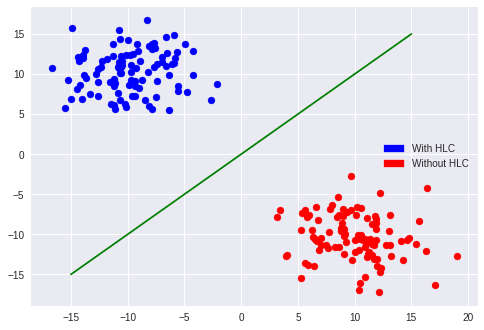
\includegraphics[width=0.7\textwidth]{graphics/linear_separation}
    \caption{Trained linear classifier on a 2-dimensional space}
    \label{fig:scattersplit}
\end{figure}
An example of how this would look with only two dimensions is shown in Figure \ref{fig:scattersplit} Once we've successfully trained this linear classifier we can run another state $s$ through the neural network. Once the prediction has finished, we view the selected action $a$ of $s$ from the policy vector $p$ from the neural network. We view the loss of that selected action $a$. Then we apply the backpropagation algorithm up to that same layer $l_{split}$ and evaluate the gradient there. If that gradient moves to the direction of the HLC we say that the state includes the HLC, and doesn't if it move away from the HLC.
\begin{figure}[]
    \centering
    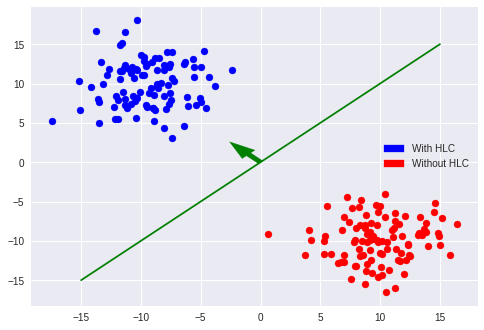
\includegraphics[width=0.7\textwidth]{graphics/linear_separation_with_direction}
    \caption{Trained linear classifier on a 2-dimensional space with arrow representing gradient}
    \label{fig:scattersplitarrow}
\end{figure}
We show an example in Figure \ref{fig:scattersplitarrow}. where the arrow in the image represents the direction the gradient is moving, if it moves toward the HLC the state $s$ includes the HLC otherwise it does not. Using this method we evaluate the internal representation of the state within the neural network, and are able to see whether it recognizes the HLC. 


